\chapter{Schlussfolgerung und Ausblick}
\label{Conclusion}
%Was wurde in dieser Arbeit gemacht? Was sind die wesentlichen Ergebnisse? Wo ist weiterer Forschungsbedarf? Welche interessanten Forschungsbereiche ergeben sich aus der eigenen Arbeit?

In dieser Arbeit wurde eine Parameterstudie zur Untersuchung von Stößen auf isotropen Platten durchgeführt. Zuerst wurde die benötigte Theorie in Kapitel~\ref{chap:Principles} hergeleitet. Anschließend wurden im Rahmen der Studie die Parameter in Tabelle~\ref{tab:VariierteParams} ausgehend vom Ausgangsfall in Tabelle~\ref{tab:Ausgang} variiert. In Kapitel~\ref{chap:Implementation} wurden die Veränderungen im Skript dargestellt und die Funktionsweise des Programmes erklärt. 

\begin{table}[H]
	\begin{center}
		\caption{Parameterstudie}
		\label{tab:VariierteParams}
		\begin{tabular}{l|c}
			\textbf{Variable} & \textbf{Wert}\\
			\hline
			$h$ & Höhe der Platte [cm]\\
			$v_{0}$ & Geschwindigkeit der Impaktors [cm/s]\\
			$r_{g}$ & Radius des Impaktors [cm]\\
			$\frac{\xi}{a}$ & Auftreffstelle in x-Richtung [entdimensioniert]\\
			$\frac{\eta}{b}$ & Auftreffstelle in y-Richtung [entdimensioniert]\\
			$Sv$ & $\frac{a}{b} \equiv \; \mbox{Seitenverhältnis der Platte}$ \\		
		\end{tabular}
	\end{center}
\end{table}

Wie in Kaptitel~\ref{chap:Durchfuehrung} ausgeführt, lassen sich einige Schlussfolgerungen aus den gewonnenen Ergebnissen ziehen. \\

Im Wesentlichen lässt sich sagen, dass die Plattensteifigkeit einen großen Einfluss auf das Verhalten der Platte hat. Allgemein lässt sich feststellen, dass eine erhöhte Plattensteifigkeit zu einer geringen Anzahl von Aufschlägen führt.

Einerseits führt eine Vergrößerung der Höhe der Platte zu einer erhöhten Steifigkeit und somit zu einer geringeren Durchbiegung und erhöhten maximalen Kraft. Hier liegt ein Kraftunterschied von $P(Mr_{max}) \; \approx \; 8 \cdot P(Mr_{min})$ vor. Dies ist auf die Potenz der Höhe in $\overline{a}$ in Kapitel~\ref{chap:Principles} zurückzuführen.

Wenn jedoch das Seitenverhältnis verändert wird, dominiert die kürzere der beiden Seiten das Verhalten der Platten. Zunächst steigt ebenfalls die maximale Kraft so wie die maximale Durchbiegung der Platte. Ab einem Seitenverhältnis von $2.5$ fallen jedoch beide kontinuierlich ab.

Betrachtet man die Geschwindigkeit des Impaktors, wird schnell ersichtlich, dass hier $v_{0}$ der dominierende Parameter ist. Zwar steigt die Auslenkung mit größer werdendem $Mr$ an, jedoch ist diese Änderung wesentlich kleiner als der Anstieg bei konstantem $Mr$ und größer werdender Geschwindigkeit. Die maximale Auslenkung und maximale Kraft zeigen einen linearen Zusammenhang bei einer Veränderung der Geschwindigkeit des Impaktors. Somit führt eine erhöhte Geschwindigkeit stets zu einer erhöhten Kraft und erhöhten maximalen Durchbiegung.

Der Radius der Kugel hat nur einen verschwindend geringen Einfluss auf die Auslenkung der Platte. Wie in Kapitel~\ref{chap:Durchfuehrung}, Abbildung~\ref{fig:RadiusAuslenkung} zu sehen ist, steigert sich die Auslenkung von $r_{g,min}$ zu $r_{g,max}$ nur in der zweiten Nachkommastelle.
Betrachtet man die maximal auftretende Kraft, sieht man, dass hier die Höhe und die Geschwindigkeit den größten Einfluss haben. Aus Abbildung~\ref{fig:Faktoren}(b) kann man ablesen, dass die Faktoren des Radius, analog zur Auslenkung, zwischen der minimalen und maximalen Kraft bei $Mr_{min}$ und $Mr_{max}$ verglichen mit den Faktoren der Höhe und der Geschwindigkeit gering sind. \\

Einen großen Einfluss auf die maximale Kraft und Durchbiegung zeigt der Aufschlagsort.
Die Anzahl der Schläge ist direkt mit dem Abstand zum Rand der Platte beziehungsweise mit dem Abstand zum Mittelpunkt der Platte verknüpft. Mit steigender Steifigkeit zum Rand hin, sinkt die maximale Anzahl an Schlägen. Jedoch sind weder die maximale Kraft noch die maximale Durchbiegung in der Mitte der Platte vorzufinden sondern breiten sich ringförmig um die Mitte der Platte aus.


\begin{figure}[H]%
	\centering
	\subfloat[Faktoren der Auslenkung]{{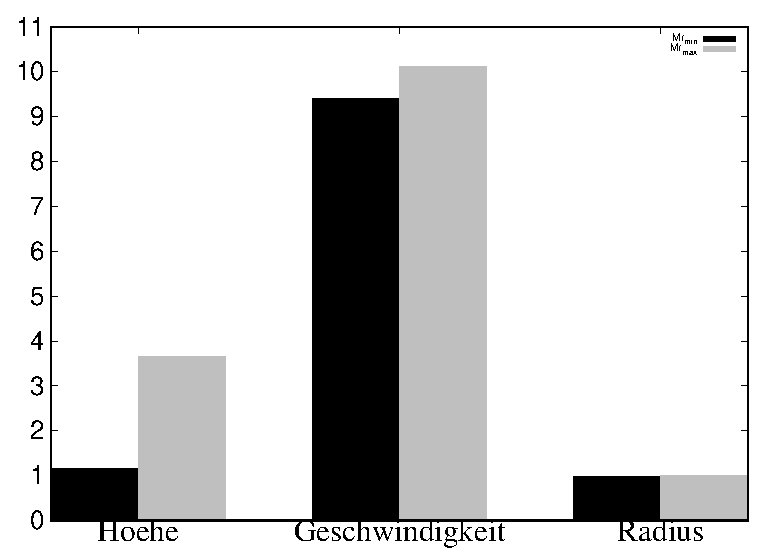
\includegraphics[width=0.4\linewidth]{pictures/gnuplot/3d/Hoehe/production/Auslenkungsfakt.eps} }}%
	\qquad
	\subfloat[Faktoren der Kraft]{{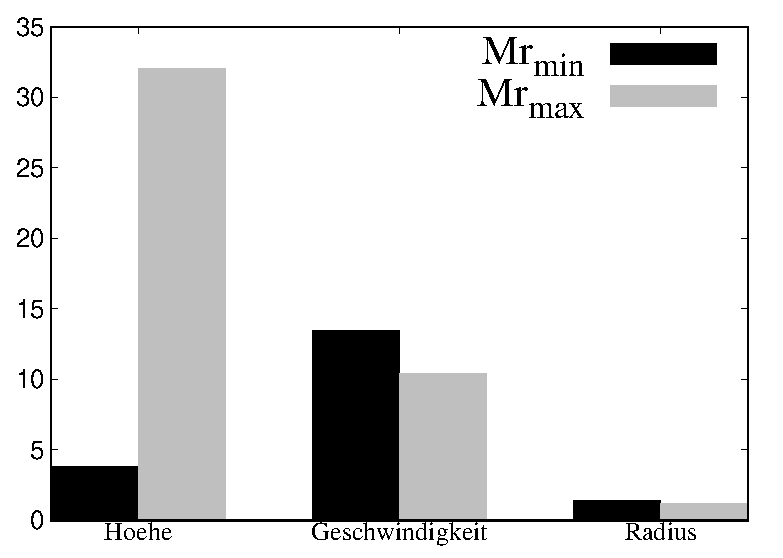
\includegraphics[width=0.4\linewidth]{pictures/gnuplot/3d/Hoehe/production/Kraftfakt.eps} }}%
	\caption{Faktoren: (v.L.n.R) Höhe, Geschwindigkeit und Radius}%
	\label{fig:Faktoren}%
\end{figure}



\section{Ausblick}
\label{sec:Ausblick}

Wie in dieser Arbeit beschrieben, haben vor allem die Plattenhöhe, die Auftreffgeschwindigkeit und die Auftreffstelle einen großen Einfluss auf das beschriebene Problem. Bei der Schadensbeurteilung sollten diese drei Faktoren berücksichtigt werden. Auch das Seitenverhältnis $Sv$ hat einen signifikanten Einfluss, jedoch sind die Ergebnisse durch die auftretenden numerischen Instabilitäten nur bedingt verlässlich. In diesem Bereich kann in zukünftigen Arbeiten weitere Recherche betrieben werden. \\
Ein weiteres Forschungsthema liegt in dem Bereich der dünnen Platten mit $h \leq 0.5 [cm]$. Eine Verfeinerung der Schrittweite könnte Platten mit $h \leq 0.5 [cm]$ auflösen, jedoch würde der zeitliche Anspruch deutlich steigen. Da oftmals dünne Platten aus Gewichtsgründen verbaut werden, sind hier weitere Überlegungen gefragt. \\
Ebenfalls wurde weder auf die maximale Spannung noch auf Queer- und Membrankräfte in der Platte eingegangen, so dass hier weitere Recherchen nötig sind.

Wie bereits in der Auswertung des Seitenverhältnisses ersichtlich, wurden Membrankräfte vernachlässigt. Dies führt zu deutlich höheren Durchbiegungen als die Realität bieten könnte.
Ein nicht-linearer Ansatz könnte dieses Problem beheben, jedoch würde die Berechnung durch gegebene Finite-Elemente Methoden oder ähnliche erheblich mehr Zeit in Anspruch nehmen und weisen qualitativ die gleiche Lösung auf.

